\documentclass[a4paper, 12pt]{article}

% packages
\usepackage{amssymb}
\usepackage[fleqn]{mathtools}
\usepackage{tikz}
\usepackage{enumerate}
\usepackage{bussproofs}
\usepackage{xcolor}
\usepackage[margin=1.3cm]{geometry}
\usepackage{logicproof}
\usepackage{diagbox}
\usepackage{listings}
\usepackage{graphicx}
\usepackage{lstautogobble}
\usepackage{hyperref}
\usepackage{multirow}
\usepackage{tipa}
\usepackage{pgfplots}
\usepackage{adjustbox}

% tikz libraries
\usetikzlibrary{
    decorations.pathreplacing,
    arrows,
    shapes,
    shapes.gates.logic.US,
    circuits.logic.US,
    calc,
    automata,
    positioning,
    intersections
}

\pgfplotsset{compat=1.16}

\pgfmathdeclarefunction{gauss}{2}{%
  \pgfmathparse{1/(#2*sqrt(2*pi))*exp(-((x-#1)^2)/(2*#2^2))}%
}

\allowdisplaybreaks % allow environments to break
\setlength\parindent{0pt} % no indent

% shorthand for verbatim
% this clashes with logicproof, so maybe fix this at some point?
\catcode`~=\active
\def~#1~{\texttt{#1}}

% code listing
\lstdefinestyle{main}{
    numberstyle=\tiny,
    breaklines=true,
    showspaces=false,
    showstringspaces=false,
    tabsize=2,
    numbers=left,
    basicstyle=\ttfamily,
    columns=fixed,
    fontadjust=true,
    basewidth=0.5em,
    autogobble,
    xleftmargin=3.0ex,
    mathescape=true
}
\newcommand{\dollar}{\mbox{\textdollar}} %
\lstset{style=main}

% augmented matrix
\makeatletter
\renewcommand*\env@matrix[1][*\c@MaxMatrixCols c]{%
\hskip -\arraycolsep
\let\@ifnextchar\new@ifnextchar
\array{#1}}
\makeatother

% ceiling / floor
\DeclarePairedDelimiter{\ceil}{\lceil}{\rceil}
\DeclarePairedDelimiter{\floor}{\lfloor}{\rfloor}

% custom commands
\newcommand{\indefint}[2]{\int #1 \, \mathrm{d}#2}
\newcommand{\defint}[4]{\int_{#1}^{#2} #3 \, \mathrm{d}#4}
\newcommand{\pdif}[2]{\frac{\partial #1}{\partial #2}}
\newcommand{\dif}[2]{\frac{\mathrm{d}#1}{\mathrm{d}#2}}
\newcommand{\limit}[2]{\raisebox{0.5ex}{\scalebox{0.8}{$\displaystyle{\lim_{#1 \to #2}}$}}}
\newcommand{\limitsup}[2]{\raisebox{0.5ex}{\scalebox{0.8}{$\displaystyle{\limsup_{#1 \to #2}}$}}}
\newcommand{\summation}[2]{\sum\limits_{#1}^{#2}}
\newcommand{\product}[2]{\prod\limits_{#1}^{#2}}
\newcommand{\intbracket}[3]{\left[#3\right]_{#1}^{#2}}
\newcommand{\laplace}{\mathcal{L}}
\newcommand{\fourier}{\mathcal{F}}
\newcommand{\mat}[1]{\boldsymbol{#1}}
\renewcommand{\vec}[1]{\boldsymbol{#1}}
\newcommand{\rowt}[1]{\begin{bmatrix}
    #1
\end{bmatrix}^\top}
\DeclareMathOperator*{\argmax}{argmax}
\DeclareMathOperator*{\argmin}{argmin}

\newcommand{\lto}[0]{\leadsto\ }

\newcommand{\ulsmash}[1]{\underline{\smash{#1}}}

\newcommand{\powerset}[0]{\wp}
\renewcommand{\emptyset}[0]{\varnothing}

\makeatletter
\newsavebox{\@brx}
\newcommand{\llangle}[1][]{\savebox{\@brx}{\(\m@th{#1\langle}\)}%
  \mathopen{\copy\@brx\kern-0.5\wd\@brx\usebox{\@brx}}}
\newcommand{\rrangle}[1][]{\savebox{\@brx}{\(\m@th{#1\rangle}\)}%
  \mathclose{\copy\@brx\kern-0.5\wd\@brx\usebox{\@brx}}}
\makeatother
\newcommand{\lla}{\llangle}
\newcommand{\rra}{\rrangle}
\newcommand{\la}{\langle}
\newcommand{\ra}{\rangle}
\newcommand{\crnr}[1]{\text{\textopencorner} #1 \text{\textcorner}}
\newcommand{\bnfsep}[0]{\ |\ }
\newcommand{\concsep}[0]{\ ||\ }

\newcommand{\axiom}[1]{\AxiomC{#1}}
\newcommand{\unary}[1]{\UnaryInfC{#1}}
\newcommand{\binary}[1]{\BinaryInfC{#1}}
\newcommand{\trinary}[1]{\TrinaryInfC{#1}}
\newcommand{\quaternary}[1]{\QuaternaryInfC{#1}}
\newcommand{\quinary}[1]{\QuinaryInfC{#1}}
\newcommand{\dproof}[0]{\DisplayProof}
\newcommand{\llabel}[1]{\LeftLabel{\scriptsize #1}}
\newcommand{\rlabel}[1]{\RightLabel{\scriptsize #1}}

\newcommand{\ttbs}{\char`\\}
\newcommand{\lrbt}[0]{\ \bullet\ }

% colours
\newcommand{\violet}[1]{\textcolor{violet}{#1}}
\newcommand{\blue}[1]{\textcolor{blue}{#1}}
\newcommand{\red}[1]{\textcolor{red}{#1}}
\newcommand{\teal}[1]{\textcolor{teal}{#1}}

% reasoning proofs
\usepackage{ltablex}
\usepackage{environ}
\keepXColumns
\NewEnviron{reasoning}{
    \begin{tabularx}{\textwidth}{rlX}
        \BODY
    \end{tabularx}
}
\newcommand{\proofline}[3]{$(#1)$ & $#2$ & \hfill #3 \smallskip \\}
\newcommand{\proofarbitrary}[1]{& take arbitrary $#1$ \smallskip \\}
\newcommand{\prooftext}[1]{\multicolumn{3}{l}{#1} \smallskip \\}
\newcommand{\proofmath}[3]{$#1$ & = $#2$ & \hfill #3 \smallskip \\}
\newcommand{\prooftherefore}[1]{& $\therefore #1$ \smallskip \\}
\newcommand{\proofbc}[0]{\prooftext{\textbf{Base Case}}}
\newcommand{\proofis}[0]{\prooftext{\textbf{Inductive Step}}}

% ER diagrams
\newcommand{\nattribute}[4]{
    \node[draw, state, inner sep=0cm, minimum size=0.2cm, label=#3:{#4}] (#1) at (#2) {};
}
\newcommand{\mattribute}[4]{
    \node[draw, state, accepting, inner sep=0cm, minimum size=0.2cm, label=#3:{#4}] (#1) at (#2) {};
}
\newcommand{\dattribute}[4]{
    \node[draw, state, dashed, inner sep=0cm, minimum size=0.2cm, label=#3:{#4}] (#1) at (#2) {};
}
\newcommand{\entity}[3]{
    \node[] (#1-c) at (#2) {#3};
    \node[inner sep=0cm] (#1-l) at ($(#1-c) + (-1, 0)$) {};
    \node[inner sep=0cm] (#1-r) at ($(#1-c) + (1, 0)$) {};
    \node[inner sep=0cm] (#1-u) at ($(#1-c) + (0, 0.5)$) {};
    \node[inner sep=0cm] (#1-d) at ($(#1-c) + (0, -0.5)$) {};
    \draw
    ($(#1-c) + (-1, 0.5)$) -- ($(#1-c) + (1, 0.5)$) -- ($(#1-c) + (1, -0.5)$) -- ($(#1-c) + (-1, -0.5)$) -- cycle;
}
\newcommand{\relationship}[3]{
    \node[] (#1-c) at (#2) {#3};
    \node[inner sep=0cm] (#1-l) at ($(#1-c) + (-1, 0)$) {};
    \node[inner sep=0cm] (#1-r) at ($(#1-c) + (1, 0)$) {};
    \node[inner sep=0cm] (#1-u) at ($(#1-c) + (0, 1)$) {};
    \node[inner sep=0cm] (#1-d) at ($(#1-c) + (0, -1)$) {};
    \draw
    ($(#1-c) + (-1, 0)$) -- ($(#1-c) + (0, 1)$) -- ($(#1-c) + (1, 0)$) -- ($(#1-c) + (0, -1)$) -- cycle;
}

% AVL Trees
\newcommand{\avltri}[4]{
    \draw ($(#1)$) -- ($(#1) + #4*(0.5, -1)$) -- ($(#1) + #4*(-0.5, -1)$) -- cycle;
    \node at ($(#1) + #4*(0, -1) + (0, 0.5)$) {#3};
    \node at ($(#1) + #4*(0, -1) + (0, -0.5)$) {#2};
}

% RB Trees
\tikzset{rbtr/.style={inner sep=2pt, circle, draw=black, fill=red}}
\tikzset{rbtb/.style={inner sep=2pt, circle, draw=black, fill=black}}

% Samples
\tikzset{spos/.style={inner sep=2pt, circle, draw=black, fill=blue!20}}
\tikzset{sneg/.style={inner sep=2pt, circle, draw=black, fill=red!20}}

% actual document
\begin{document}
    {\sc Computing $3^\text{rd}$ Year Notes} \hfill ~https://github.com/lin-e/imperial-revision~
    \rule{\textwidth}{0.1pt}
    \section*{CO572 - Advanced Databases \hfill (60002)}
        \subsection*{Lecture 1}
            What is a \textbf{database management system}?
            A \textbf{database} is any structured collection of data points, which can be a relational table, a set, a vector, a graph, or anything along those lines.
            \textbf{Data management} is needed for \textbf{data-intensive applications}, we say something processes a significant amount of data if the amount of data is larger than what fits in the CPU's cache, something in the order of a few MB.
            We can say that below this threshold (around 5MB - 50MB), there are other factors that likely dominate performance.
            A \textbf{system} is made up from components that interact together to achieve a greater goal and is usually applicable to many situations.
            \subsubsection*{Applications}
                \begin{itemize}
                    \itemsep0em
                    \item
                        The scenario is at a hospital.
                        At any given time, there are 800 patients, producing a sample per second of 5 metrics.
                        There are also 200 doctors and nurses, who each produce a textual report every 10 minutes, and 80 lab technicians producing a structured dataset of 10 metrics every 5 minutes.
                        Everything must be stored \textbf{reliably}, it cannot be lost after it is stored (or with a probability $p < 0.001$).
                    \item
                        You are developing a interactive dashboard for a global retail company.
                        This company has stored 500GBs of sales, inventory, and customer records, and shall provide interactive access to calculated statistics.
                        This should allow filtering of the dataset with predicates, and support the calculation of the sums of records, all with response times below a second.
                \end{itemize}
                Below are some examples of typical data-intensive application patterns;
                \begin{itemize}
                    \itemsep0em
                    \item Online Transaction Processing \hfill \textbf{OLTP}
                        \begin{itemize}
                            \itemsep0em
                            \item lots of small updates to a persistent database
                            \item focused on throughput (do as many updates as possible in a time-frame)
                            \item ACID is key (reliable)
                        \end{itemize}
                    \item Online Analytical Processing \hfill \textbf{OLAP}
                        \begin{itemize}
                            \itemsep0em
                            \item running a single data analysis task
                            \item focus on latency (do queries as quickly as possible)
                            \item \textbf{ad-hoc} queries - we don't know what they'll be
                        \end{itemize}
                    \item Reporting
                        \begin{itemize}
                            \itemsep0em
                            \item running many analysis tasks in a fixed time budget
                            \item focused on resource efficiency - if we can do the same task by the same time it's due with fewer resources, then it would be cheaper
                            \item queries are known in advance (and can be compiled into the system)
                        \end{itemize}
                    \item Hybrid Transactional / Analytical Processing \hfill \textbf{HTAP}
                        \begin{itemize}
                            \itemsep0em
                            \item a mix of \textbf{OLTP} and \textbf{OLAP}
                            \item small updates woven with larger analytics
                            \item common application is fraud detection
                        \end{itemize}
                \end{itemize}
            \subsubsection*{Data-intensive Application vs Management System}
                A \textbf{application} is not generic - it's often domain-specific with the logic baked in, and is therefore hard to generalise to other applications.
                Generally, the cost (such as adapting for other applications) of application-specific data management outweighs the benefits.
                We can generalise the following (from an application to a management system);
                \begin{itemize}
                    \itemsep0em
                    \item \textit{Yelp}
                    \item mobile app for geo-services
                    \item library to manage unordered collections of tagged coordinates
                    \item spatial data management library
                    \item relational database
                    \item block storage system
                \end{itemize}
            \subsubsection*{Requirements of a Data Management System}
                A data management system should fulfil the following requirements;
                \begin{itemize}
                    \itemsep0em
                    \item \textbf{efficiency} \hfill should not be significantly slower than hand written applications
                    \item \textbf{resilience} \hfill should recover from problems, such as power outage, hardware or software failures
                    \item \textbf{robustness}
                        \subitem should have predictable performance; a small change in the query should not lead to major changes in performance
                    \item \textbf{scalability}
                        \subitem should make efficient use of available resources - increase in resources should lead to an improvement of performance
                    \item \textbf{concurrency}
                        \subitem should transparently serve multiple clients transparently (without impacting results)
                \end{itemize}
            \subsubsection*{Solutions}
                DBMSs often provide some ingenious solutions;
                \begin{itemize}
                    \itemsep0em
                    \item \textbf{Physical and Logical Data Model Separation}
                        \subitem
                            We typical provide a \textbf{logical data model} to the user, as they often send data in a \textbf{fire and forget} manner.
                            The user doesn't typically care about file format, storage devices, nor portability.
                            The DMBSs can then separate external from the internal model and therefore exploit these degrees of freedom for performance.
                            For example, if the user doesn't care where the data is stored, we can keep the hot data on an SSD and the cold data on disk or even tape.
                    \item \textbf{Transparent Concurrency: Transactional Semantics}
                        \begin{itemize}
                            \itemsep0em
                            \item \textbf{Atomic} \hfill run completely or not at all (if aborted, everything is reverted)
                            \item \textbf{Consistent} \hfill constraints must hold before and after (can be inconsistent between)
                            \item \textbf{Isolated} \hfill run like you were alone on the system
                            \item \textbf{Durable} \hfill after a transaction is committed \textbf{nothing} can undo it
                        \end{itemize}
                    \item \textbf{Ease of Use: Declarative Data Analysis}
                        \subitem
                            Retrieving information about data should be done by describing the result and the system will generate it.
                            This can be a single tuple, some statistics, a detailed generated report, or even training a model to predict data.
                \end{itemize}
                However, they are not to be used as a filesystem.
                Similarly, it cannot be used as runtime for applications - there are support for user-defined functions, but should not be used a such.
                They also should not be used to store intermediate data (such as whether a user is logged in).
            \subsubsection*{Relational Algebra}
                A schema is the definition of the attributes of the tuples in the relations, but also can contain integrity constraints.
                \begin{itemize}
                    \itemsep0em
                    \item \textbf{vector} \hfill ordered collection of objects of the same type
                    \item \textbf{tuple} \hfill ordered collection of objects of different type
                    \item \textbf{bag} \hfill unordered collection of objects of the same type
                    \item \textbf{set} \hfill unordered collection of unique objects of the same type
                \end{itemize}
                Relational algebra is used to define the semantics of operations and is used for logical optimisation.
                However, it's not actually that useful for end-users.
                A relation is an array which represents an $n$-ary relation $R$, with the following properties;
                \begin{itemize}
                    \itemsep0em
                    \item each row represents an $n$-tuple of $R$
                    \item the order of rows doesn't matter
                    \item all rows are distinct (combined with above is a set)
                    \item the order of columns matters - all rows have the same schema
                    \item each column has a label (defines the schema of our relation)
                \end{itemize}
                Relations are \textbf{almost} sets of tuples.
                A rough implementation in C++ is as follows;
                \begin{lstlisting}
                    template <typename... types>
                    struct Relation {
                        using OutputType = tuple<types...>;
                        set<tuple<types...>> data;
                        array<string, sizeof...(types)> schema;
                        Relation(){};
                        Relation(array<string, sizeof...(types)> schema, set<tuple<types...>> data): schema(schema), data(data) {}
                    };
                \end{lstlisting}
                A relation can then be written as follows;
                \begin{lstlisting}
                    auto createCustomerTable() {
                        Relation<int, string, string> customer(
                            {"ID", "Name", "ShippingAddress"}, // labels of the attribute
                            {{1, "james", "address 1"},
                             {2, "steve", "another address}});
                        return customer;
                    }
                \end{lstlisting}
                A \textbf{relational expression} is composed from \textbf{relational operators}, and will often be referred to as a \textbf{(logical) plan}.
                \textbf{Cardinality} is the number of tuples in a set.
                Relational operations are set-based, and therefore order-invariant and duplicates are eliminated.
                Additionally, it's \textbf{closed};
                \begin{itemize}
                    \itemsep0em
                    \item every operator produces a relation as an output
                    \item every operator accepts one or two relations as input
                    \item simplifies the composition of operators into expressions (however expressions can be invalid)
                \end{itemize}
                Relational operators can be implemented as follows;
                \begin{lstlisting}
                    template <typename... types> struct Operator : public Relation<types...> {}; // therefore an operator is a relation
                \end{lstlisting}
                A minimal set of relational operators is as follows;
                \begin{itemize}
                    \itemsep0em
                    \item \textbf{project} ($\pi$)
                        \begin{itemize}
                            \itemsep0em
                            \item extract one or more attributes from a relation
                            \item preserves relational semantics
                            \item changes schema
                        \end{itemize}
                        For example, given a table;
                        \begin{center}
                            \hfill
                            \begin{tabular}{ccc}
                                \multicolumn{3}{c}{~table1~} \\
                                ~field1~ & ~field2~ & ~field3~ \\
                                \hline
                                ~A~ & ~B~ & ~C~ \\
                                ~D~ & ~E~ & ~F~ \\
                                ~G~ & ~E~ & ~I~
                            \end{tabular}
                            \hfill
                            \begin{tabular}{c}
                                \multicolumn{1}{c}{$\pi_~field2~~table1~$} \\
                                ~field2~ \\
                                \hline
                                ~B~ \\
                                ~E~ \\
                                \phantom{}
                            \end{tabular}
                            \hfill \phantom{}
                        \end{center}
                        The cardinality of the output of a projection can only be determined by evaluating it, as duplicates can be eliminated.
                        On the other hand, the upper bound of the cardinality of the output is the cardinality of the input.
                        \medskip

                        It can also extract one or more attributes from a relation and perform a scalar operation on them.
                        \begin{lstlisting}
                            template <typename InputOperator, typename... outputTypes>
                            struct Project : public Operator<outputTypes...> {
                                InputOperator input;

                                variant<function<tuple<outputTypes...>(typename InputOperator::OutputType)>,
                                        set<pair<string, string>>>
                                    projections;

                                Project(InputOperator input, function<tuple<outputTypes...>(typename InputOperator::OutputType)> projections : input(input), projections(projections) {};

                                Project(InputOperator input, set<pair<string, string>> projections : input(input), projections(projections) {};
                            };

                            void projectionExample {
                                auto customer = createCustomerTable();

                                auto p1 = Project<decltype(customer), string>(customer, [](auto input) { return get<1>(input); });

                                auto p2 = Project<decltype(customer), string>(customer, {{"Name", "customerName"}});
                            }
                        \end{lstlisting}
                    \item \textbf{select} ($\sigma$)
                        \begin{itemize}
                            \itemsep0em
                            \item produces a new relation containing tuples which satisfy a condition
                            \item does not change schema
                            \item changes cardinality (number of tuples in a relation)
                        \end{itemize}
                        For example, given a table;
                        \begin{center}
                            \hfill
                            \begin{tabular}{ccc}
                                \multicolumn{3}{c}{~table1~} \\
                                ~field1~ & ~field2~ & ~field3~ \\
                                \hline
                                ~A~ & ~B~ & ~C~ \\
                                ~D~ & ~E~ & ~F~ \\
                                ~G~ & ~E~ & ~I~
                            \end{tabular}
                            \hfill
                            \begin{tabular}{ccc}
                                \multicolumn{3}{c}{$\sigma_~field2=E~~table1~$} \\
                                ~field1~ & ~field2~ & ~field3~ \\
                                \hline
                                ~D~ & ~E~ & ~F~ \\
                                ~G~ & ~E~ & ~I~ \\
                                \phantom{}
                            \end{tabular}
                            \hfill \phantom{}
                        \end{center}
                        The cardinality can only be determined by evaluating it, and the upper bound of the cardinality is also the cardinality of the input.
                        \begin{lstlisting}
                            enum class Comparator { less, lessEqual, equal, greaterEqual, greater };

                            struct Column {
                                string name;
                                Column(string name) : name(name) {};
                            };
                            using Value = variant<string, int float>;

                            struct Condition {
                                Column leftHandSide;
                                Comparator compare;
                                variant<Column, Value> rightHandSide;

                                Condition(Column leftHandSide, Comparator compare, variant<Column, Value> rightHandSide): leftHandSide(leftHandSide), compare(compare), rightHandSide(rightHandSide) {};
                            };
                        \end{lstlisting}
                    \item \textbf{cross product} ($\times$)
                        \begin{itemize}
                            \itemsep0em
                            \item takes two inputs
                            \item produces a new relation by combining every tuple from the left with every tuple from the right
                            \item changes the schema
                        \end{itemize}
                        For example, given tables;
                        \begin{center}
                            \hfill
                            \begin{tabular}{ccc}
                                \multicolumn{2}{c}{~table1~} \\
                                ~field1~ & ~field2~ \\
                                \hline
                                ~A~ & ~B~ \\
                                ~G~ & ~E~ \\
                                \phantom{} \\
                                \phantom{}
                            \end{tabular}
                            \hfill
                            \begin{tabular}{ccc}
                                \multicolumn{2}{c}{~table2~} \\
                                ~fieldA~ & ~fieldB~ \\
                                \hline
                                ~2~ & ~6~ \\
                                ~5~ & ~1~ \\
                                \phantom{} \\
                                \phantom{}
                            \end{tabular}
                            \hfill
                            \begin{tabular}{cccc}
                                \multicolumn{4}{c}{$~table1~ \times ~table2~$} \\
                                ~field1~ & ~field2~ & ~fieldA~ & ~fieldB~ \\
                                \hline
                                ~A~ & ~B~ & ~2~ & ~6~ \\
                                ~A~ & ~B~ & ~5~ & ~1~ \\
                                ~G~ & ~E~ & ~2~ & ~6~ \\
                                ~G~ & ~E~ & ~5~ & ~1~
                            \end{tabular}
                            \hfill \phantom{}
                        \end{center}
                        The cardinality of the output is the product of the two input cardinalities.
                        \begin{lstlisting}
                            template <typename LeftInputOperator, typename RightInputOperator>
                            struct CrossProduct : public Operator<Concat<typename LeftInputOperator::OutputType, typename RightOutputOperator::OutputType>> {
                                LeftInputOperator leftInput;
                                RightInputOperator rightInput;
                                CrossProduct(LeftInputOperator leftInput, RightInputOperator  rightInput): leftInput(leftInput), rightInput(rightInput) {};
                            };
                        \end{lstlisting}
                    \item \textbf{union} ($\cup$)
                        \begin{itemize}
                            \itemsep0em
                            \item produces a new relation from two relations containing any tuple that is present in either
                            \item does not change the schema (but does require schema compatibility)
                            \item changes cardinality
                        \end{itemize}
                        No example provided, because it's quite simple.
                        \begin{lstlisting}
                            template <typename LeftInputOperator, typename RightInputOperator>
                            struct Union : public Operator<typename LeftInputOperator:::OutputType> {
                                LeftInputOperator leftInput;
                                RightInputOperator rightInput;

                                Union(LeftInputOperator leftInput, RightInputOperator rightInput): leftInput(leftInput), rightInput(rightInput){};
                            };
                        \end{lstlisting}
                        The cardinality can only be known by evaluating (due to duplicates), and the upper bound is the sum of the cardinalities of the input.
                    \item \textbf{difference} ($-$)
                        \begin{itemize}
                            \itemsep0em
                            \item produces new relation from two relations containing tuples present in the first but not the second
                            \item doesn't change schema (requires compatibility)
                            \item changes cardinality
                        \end{itemize}
                        No example provided, because it's quite simple.
                        \begin{lstlisting}
                            template <typename LeftInputOperator, typename RightInputOperator>
                            struct Difference : public Operator<typename LeftInputOperator:::OutputType> {
                                LeftInputOperator leftInput;
                                RightInputOperator rightInput;

                                Difference(LeftInputOperator leftInput, RightInputOperator rightInput): leftInput(leftInput), rightInput(rightInput){};
                            };
                        \end{lstlisting}
                    \item \textbf{group aggregation} ($\Gamma$)
                        \begin{itemize}
                            \itemsep0em
                            \item produces new relation from one input by grouping tuples that have equal values in some attributes and aggregate others - groups are defined by the set of grouping attributes (can be empty), and the aggregates are defined by the set of \textbf{aggregations} which are triples consisting of;
                                \begin{itemize}
                                    \itemsep0em
                                    \item \textbf{input} attribute
                                    \item \textbf{aggregation function} (min, max, avg, sum, count)
                                    \item \textbf{output} attribute
                                \end{itemize}
                            \item this changes both the schema and cardinality
                        \end{itemize}
                        For example, given the following table;
                        \begin{center}
                            \hfill
                            \begin{tabular}{ccc}
                                \multicolumn{3}{c}{~customer~} \\
                                ~ID~ & ~Name~ & ~City~ \\
                                \hline
                                ~1~ & ~james~ & ~London~ \\
                                ~2~ & ~steve~ & ~London~ \\
                                ~3~ & ~kate~ & ~Manchester~
                            \end{tabular}
                            \hfill
                            \begin{tabular}{cc}
                                \multicolumn{2}{c}{$\Gamma((~City~),((~ID~,~count~,~c~)))~Customer~$} \\
                                ~City~ & ~c~ \\
                                \hline
                                ~London~ & ~2~ \\
                                ~Manchester~ & ~1~ \\
                                \phantom{}
                            \end{tabular}
                            \hfill
                            \phantom{}
                        \end{center}
                        \begin{lstlisting}
                            enum class AggregationFunction { min, max, sum, avg, count };

                            template <typename InputOperator, typename... Output>
                            struct GroupedAggregation : public Operator<Output...> {
                                InputOperator input;
                                set<string> groupAttributes;
                                set<tuple<string, AggregationFunction, string>> aggregations;
                                GroupedAggregation(InputOperator input, set<string> groupAttributes, set<tuple<string, AggregationFunction, string>> aggregations): input(input), groupAttributes(groupAttributes), aggregations(aggregations){};
                            };
                        \end{lstlisting}
                    \item \textbf{Top-N} ($T$)
                        \begin{itemize}
                            \itemsep0em
                            \item produce new relation from one input selecting the tuples with the $N$ greatest values with respect to an attribute
                            \item changes cardinality, but maintains schema
                        \end{itemize}
                        For example, given the following table;
                        \begin{center}
                            \hfill
                            \begin{tabular}{ccc}
                                \multicolumn{3}{c}{~customer~} \\
                                ~ID~ & ~Name~ & ~City~ \\
                                \hline
                                ~1~ & ~james~ & ~London~ \\
                                ~2~ & ~steve~ & ~London~ \\
                                ~3~ & ~kate~ & ~Manchester~
                            \end{tabular}
                            \hfill
                            \begin{tabular}{ccc}
                                \multicolumn{3}{c}{$T_{(2, ~ID~)}~Customer~$} \\
                                ~ID~ & ~Name~ & ~City~ \\
                                \hline
                                ~2~ & ~steve~ & ~London~ \\
                                ~3~ & ~kate~ & ~Manchester~ \\
                                \phantom{}
                            \end{tabular}
                            \hfill
                            \phantom{}
                        \end{center}
                        \begin{lstlisting}
                            template <typename InputOperator>
                            struct TopN : public Operator<typename InputOperator::OutputType> {
                                InputOperator input;
                                size_t N;
                                string predicate;
                                TopN(InputOperator input, size_t N, string predicate): input(input), N(N), predicate(predicate){};
                            };
                        \end{lstlisting}
                \end{itemize}
                Since relational algebra is closed, operators can be combined as long as signatures are respected (cross product takes two inputs, whereas selections and projections take one);
                $$\pi_~BookID~(\sigma_~Order.ID == OrderedItem.OrderID~(~Order~ \times ~OrderedItem~))$$
        \subsection*{Lecture 2}
            \subsubsection*{Architecture}
                The logical plan is the relational algebra discussed last lecture and the database kernel actually interacts with the resources mentioned.
                A database kernel is a library of core functionality, including I/O, memory management, operators, etc.
                Generally, it provides an interface to subsystems (similar to an OS kernel).
                A basic database kernel architecture is as follows (assuming both catalogue and data live in memory).
                \begin{center}
                    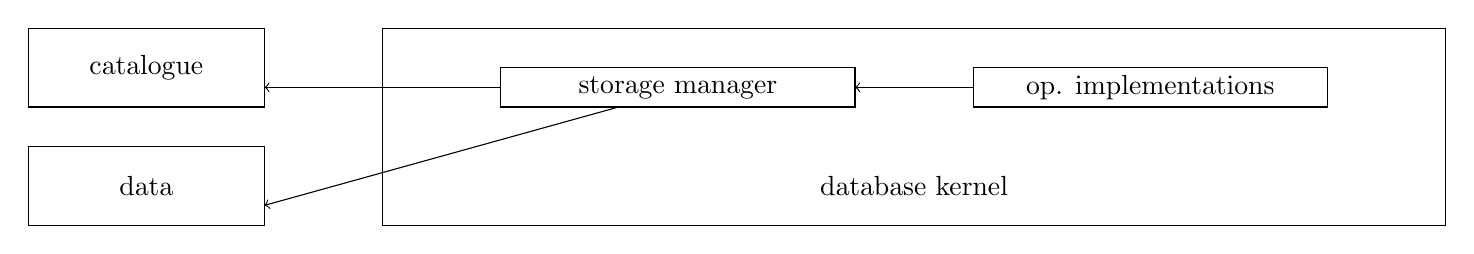
\begin{tikzpicture}[x=1.5cm, y=0.5cm]
                        \draw
                        (0, 0) -- (9, 0) -- (9, -5) -- (0, -5) -- cycle
                        (1, -1) -- (4, -1) -- (4, -2) -- (1, -2) -- cycle
                        (5, -1) -- (8, -1) -- (8, -2) -- (5, -2) -- cycle
                        (-3, 0) -- (-1, 0) -- (-1, -2) -- (-3, -2) -- cycle
                        (-3, -3) -- (-1, -3) -- (-1, -5) -- (-3, -5) -- cycle;

                        \node at (2.5, -1.5) {storage manager};
                        \node at (6.5, -1.5) {op. implementations};
                        \node at (-2, -1) {catalogue};
                        \node at (-2, -4) {data};
                        \node at (4.5, -4) {database kernel};
                        \draw
                        (5, -1.5) edge[->] (4, -1.5)
                        (1, -1.5) edge[->] (-1, -1.5)
                        (2, -2) edge[->] (-1, -4.5);
                    \end{tikzpicture}
                \end{center}
                The DBMS architecture is as follows;
                \begin{center}
                    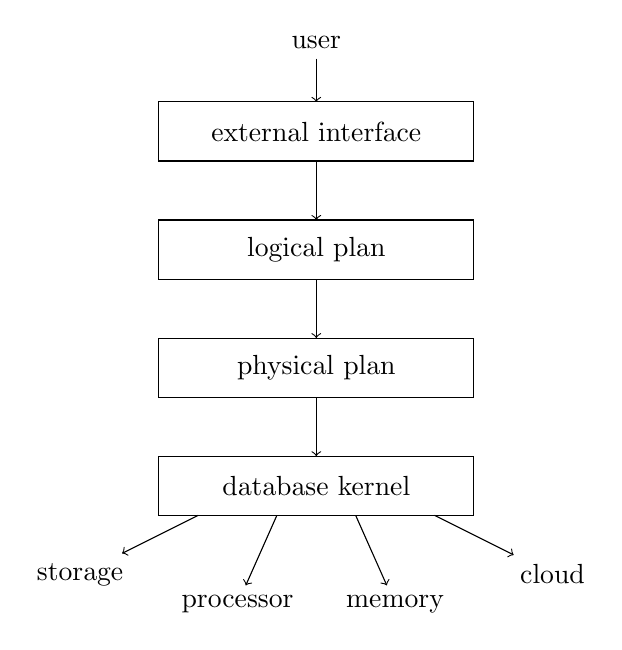
\begin{tikzpicture}[y=0.75cm]
                        \node (u) at (2, 1) {user};
                        \node at (2, -0.5) {external interface};
                        \node at (2, -2.5) {logical plan};
                        \node at (2, -4.5) {physical plan};
                        \node at (2, -6.5) {database kernel};
                        \draw (0, 0) -- (4, 0) -- (4, -1) -- (0, -1) -- cycle;
                        \draw (0, -2) -- (4, -2) -- (4, -3) -- (0, -3) -- cycle;
                        \draw (0, -4) -- (4, -4) -- (4, -5) -- (0, -5) -- cycle;
                        \draw (0, -6) -- (4, -6) -- (4, -7) -- (0, -7) -- cycle;
                        \node (storage) at (-1, -8) {storage};
                        \node (cpu) at (1, -8.5) {processor};
                        \node (mem) at (3, -8.5) {memory};
                        \node (cloud) at (5, -8) {cloud};
                        \draw
                        (u) edge[->] (2, 0)
                        (2, -1) edge[->] (2, -2)
                        (2, -3) edge[->] (2, -4)
                        (2, -5) edge[->] (2, -6)
                        (0.5, -7) edge[->] (storage)
                        (1.5, -7) edge[->] (cpu)
                        (2.5, -7) edge[->] (mem)
                        (3.5, -7) edge[->] (cloud);
                    \end{tikzpicture}
                \end{center}
                The kernel interface, in C++, would look like the following;
                \begin{lstlisting}
                    class StorageManager;
                    class OperatorImplementations;

                    // just provides an interface to the above
                    class DatabaseKernel {
                        StorageManager& getStorageManager();
                        OperatorImplementations& getOperatorImplementations();
                    }
                \end{lstlisting}
            \subsubsection*{Storage}
                The first operation every database needs to support inserting new tuples.
                These inserts are usually not optimised (generally) - they arrive at the storage layer as intact tuples.
                Consider the following example, in SQL;
                \begin{lstlisting}
                    CREATE TABLE Employee (
                        id int,
                        name varchar,
                        salary int,
                        joiningDate int
                    );

                    INSERT INTO Employee VALUES(1, 'james', 100000, 43429342);
                    SELECT * FROM Employee WHERE id=1;
                    DELETE FROM Employee WHERE name='james';
                \end{lstlisting}
                The equivalent in C++ would be as follows;
                \begin{lstlisting}
                    StorageManager().getTable("Employee").insert({1, "james", 100000, 43429342});
                    StorageManager().getTable("Employee").findTuplesWithAttributeValue(id, 4);
                    StorageManager().getTable("Employee").deleteTuplesWithAttributeValue(name, "james");
                \end{lstlisting}
                The storage manager interface would be as follows;
                \begin{lstlisting}
                    struct Table;
                    class StorageManager {
                        map<string, Table> catalogue;

                        public:
                            Table& getTable(string name) {return catalogue[name]; };
                    };
                \end{lstlisting}
                In order to store tuples, we need to decide where and how we store data.
                Generally, for where we store it, we mainly consider disk or memory.
                The way we store data can vary from being sorted, compressed, RLE-encoded, etc.
                A simple table interface could be as follows;
                \begin{lstlisting}
                    struct Table {
                        using AttributeValue = variant<int, float, string>;
                        using Tuple = vector<AttributeValue>;

                        void insert(Tuple) {};
                        vector<Tuple> findTuplesWithAttributeValue(int attributePosition, AttributeValue value) {};
                        void deleteTuplesWithAttributeValue(int attributePosition, AttributeValue value) {};
                    };
                \end{lstlisting}
                There is a fundamental mismatch in storing tuples; relations are two-dimensional, whereas memory is one-dimensional, therefore tuples need to be linearized in one of the two mainstream strategies;
                \begin{itemize}
                    \itemsep0em
                    \item \textbf{The N-ary Storage Model} (NSM)
                        \subitem
                            In this model, the entries added are stored one after the other, in a one-to-one mapping onto memory.
                            This is also referred to as a \textbf{row store}.
                            An example of this is as follows;
                            \begin{lstlisting}
                                struct NSMTable : public Table {

                                    // not the tuple exposed to the outside
                                    struct InternalTuple {
                                        Tuple actualTuple;
                                        bool deleted = false;
                                        InternalTuple(Tuple t) : actualTuple(t) {};
                                    }
                                    vector<InternalTuple> data;

                                    void insert(Tuple);
                                    vector<Tuple> findTuplesWithAttributeValue(int attributePosition, AttributeValue value) {};
                                    void deleteTuplesWithAttributeValue(int attributePosition, AttributeValue value) {};
                                };

                                // declared as member of a class (just append to a vector)
                                void NSMTable::insert(Tuple t) { data.push_back(t); }

                                vector<Table::Tuple> NSMTable::findTuplesWithAttributeValue(int attributePosition, AttributeValue value) {
                                    vector<Tuple> result;
                                    for (size_t i = 0; i < data.size(); i++) {
                                        if (data[i].actualTuple[attributePosition] == value && !data[i].deleted) {
                                            result.push_back(data[i].actualTuple);
                                        }
                                    }
                                    return result;
                                }

                                // we don't want to move everything therefore we just mark them as deleted
                                void NSMTable::deleteTuplesWithAttributeValue(int attributePosition, AttributeValue value) {
                                    for (size_t i = 0; i < data.size(); i++) {
                                        if (data[i].actualTuple[attributePosition] == value) {
                                            data[i].deleted = true;
                                        }
                                    }
                                }
                            \end{lstlisting}
                            However, this may not always be a good idea, as operations will require us going over the entire vector.
                            Recall that we are assuming everything is in memory, however locality still matters (since the data may be further apart depending on the size of the tuple).
                            \medskip

                            Memory is organised in \textbf{cache lines} (usually 64 bytes in size).
                            When a core needs something, it asks L1, L2, and L3 cache first, before going to memory, and retrieves the entire cache line that the data resides on (and cache into L1 cache).
                            If we then access something on the same cache line, then the access is almost free (in terms of time).
                            More tuples will therefore fit on a single cache line if they are smaller.
                            Cache lines can also be referred to as \textbf{blocks} or \textbf{pages}.
                            \medskip

                            N-ary storage works well in inserting a new tuple, when we are inserting a tuple onto the same cache line.
                            It also works well when we want to retrieve a tuple by its index.
                            On the other hand, it's suboptimal when we want to check every row, which in the worst case will be across different cache lines.
                    \item \textbf{Decomposed Storage Model} (DSM)
                        \subitem
                            On the other hand, in this model, entries are stored with the columns one after the other.
                            This is also referred to as \textbf{column store}.
                            An example of this implementation is as follows;
                            \begin{lstlisting}
                                struct DSMTable : public Table {
                                    using Column = vector<AttributeValue>;
                                    vector<Column> data;
                                    vector<bool> deleteMarkers;

                                    void insert(Tuple);
                                    vector<Tuple> findTuplesWithAttributeValue(int attributePosition, AttributeValue value) {};
                                    void deleteTuplesWithAttributeValue(int attributePosition, AttributeValue value) {};
                                };

                                // inserts cause tuple decomposition
                                void DSMTable::insert(Tuple tuple) {
                                    for (int i = 0; i < tuple.size(); i++) {
                                        data[i].push_back(tuple[i]);
                                    }
                                }

                                // find requires tuple reconstruction
                                vector<Table::Tuple> DSMTable::findTuplesWithAttributeValue(int attributePosition, AttributeValue value) {
                                    vector<Tuple> result;
                                    for (size_t i = 0; i < data[attributePosition].size(); i++) {
                                        if (data[attributePosition][i] == value && !deleteMarkers[i]) {
                                            Tuple reconstructedTuple;
                                            for (int column = 0; column < data.size(); column++) {
                                                reconstructedTuple.push_back(data[column][i]);
                                            }
                                            result.push_back(reconstructedTuple);
                                        }
                                    }
                                    return result;
                                }

                                void DSMTable::deleteTuplesWithAttributeValue(int attributePosition, AttributeValue value) {
                                    for (size_t i = 0; i < data.size(); i++) {
                                        if (data[attributePosition][i] == value) {
                                            deleteMarkers[i] = true;
                                        }
                                    }
                                }
                            \end{lstlisting}
                            Decomposed storage works well in the case when we are iterating over one column of a tuple.
                            However, if these entries are one after the other, there is perfect data locality, which minimises the number of cache lines we need.
                            On the other hand, insertion is suboptimal as we need to spread a tuple over memory.
                            Similarly, accessing a single tuple, even when we know where it is in memory is suboptimal, as the tuple will need to be reconstructed.
                    \item Hybrid Delta / Main Storage
                        \begin{lstlisting}
                            struct HybridTable : public Table {
                                DSMTable main; // every tuple will eventually end up here
                                NSMTable delta; // will be inserted here then merged into main

                                void insert(Tuple);
                                vector<Tuple> findTuplesWithAttributeValue(int attributePosition, AttributeValue value) {};
                                void deleteTuplesWithAttributeValue(int attributePosition, AttributeValue value) {};
                                void merge();
                            };

                            void HybridTable::insert(Tuple t) {
                                delta.insert(t);
                            }

                            vector<Table::Tuple> HybridTable::findTuplesWithAttributeValue(int attributePosition, AttributeValue value) {
                                vector<Tuple> results = main.findTuplesWithAttributeValue(attributePosition, value);
                                vector<Tuple> fromDelta = delta.findTuplesWithAttributeValue(attributePosition, value);
                                results.insert(results.end(), fromDelta.begin(), fromDelta.end());
                                return results;
                            }

                            void HybridTable::deleteTuplesWithAttributeValue(int attributePosition, AttributeValue value) {
                                main.deleteTuplesWithAttributeValue(attributePosition, value);
                                delta.deleteTuplesWithAttributeValue(attributePosition, value);
                            }

                            void HybridTable::merge() {
                                for (auto i = 0u; i < delta.data.size(); i++) {
                                    // these two operations need to atomic (otherwise we can return the same tuple multiple times)
                                    main.insert(delta.data[i].actualTuple);
                                    delta.data[i].deleted = true;
                                }
                            }
                        \end{lstlisting}
                \end{itemize}
                In conclusion, \textbf{DSM} works well fro scan-heavy queries (accessing a lot of tuples but few columns).
                This is common in analytical processing, and analytics mostly operate on historical data.
                On the other hand \textbf{NSM} works well for lookups and inserts.
                This is more common in transactional processing (inserting sales item, looking up products, etc).
                Transactions mostly operate on recent data.
                Hybrid exploits the aforementioned workloads, but it needs regular migrations (~merge()~) which may need to lock the database.
            \subsubsection*{Catalogue}
                The catalogue stores metadata.
                The idea is that real-life data follows patterns, which if recognised and exploited, can lead to more efficiency.
                However metadata will need to be stored and maintained.
                Examples of metadata can be type, min / max values (if data is requested outside a range we know it doesn't exist), histograms, etc.
                Two simple ones are \textbf{sortedness} and \textbf{denseness}.
                Consider the following example, which is a common pattern (as the first column is often IDs);
                \begin{lstlisting}
                    class Table {
                        vector<Tuple> storage;
                        bool firstColumnIsSorted = true;
                        bool firstColumnIsDense = true;

                        public:
                            void insert(Tuple t) {
                                if (storage.size() > 0) {
                                    firstColumnIsSorted &= (t[0] >= storage.back()[0]);
                                    firstColumnIsDense &= (t[0] == storage.back()[0] + 1);
                                }
                                storage.push_back(t);
                            }

                            vector<Tuple> findTuplesWithAttributeValue(int attribute, AttributeValue value) {
                                if (attribute == 0 && firstColumnIsDense) {
                                    return { data[value - storage.front()[0]] };
                                } else if (attribute == 0 && firstColumnIsSorted) {
                                    if (binary_search(data, attribute, value)[0] == value) {
                                        return { binary_search(data, attribute, value) };
                                    }
                                }
                                ... // same scan as before
                            }

                            // we can also exploit the fact that order of rows doesn't matter, and therefore we can reorganise
                            void analyse() {
                                // this sort can be expensive (and therefore should be run regularly but not always)
                                sort(storage.begin(), storage.end(), [](auto l, auto r) { return l[0] < r[0] });
                                firstColumnIsSorted = true;
                                firstColumnIsDense = true;
                                for (size_t = 1; i < storage.size(); i++) {
                                    firstColumnIsDense &= storage[i][0] == storage[i - 1][0] + 1;
                                }
                            }
                    }
                \end{lstlisting}
            \subsubsection*{Variable Length Data}
                It's important to note that strings tend to have different lengths.
                However, we'd like to maintain fixed tuple sizes, as it allows for random access to tuples by their position.
                We can either overallocate space for ~varchars~ (for example, some system require a size parameter for maximum length), or we can store them out of place.
                Overallocating leads to strings under the maximum length being padded with some sort of terminator.
                This is good for locality and is simple to implement, however it's very wasteful for space (especially if they are too generous with lengths).
                \medskip

                On the other hand, out of place storage now contain an index into a dictionary, which contains the string (all null terminated).
                However, retrieving a value will need an access to obtain the index and another to get the actual value (which has poor locality).
                While this is better for space (and is what most programming languages do), it's also complicated (and causes difficult garbage-collection).
                This gives an optimisation (\textbf{dictionary compression}) however - if we find a string that has already been used when we insert, we can use the address of the existing value for the insert.
            \subsubsection*{Data Storage on Disk}
                Disks are different from main memory in a number of ways;
                \begin{itemize}
                    \itemsep0em
                    \item \textbf{larger pages} \hfill kilobytes compared to bytes
                    \item \textbf{higher latency} \hfill milliseconds compared to nanoseconds
                    \item \textbf{lower throughput} \hfill hundreds of megabytes instead of tens of gigabytes per second
                        \subitem this is why we consider DBMSs as I/O bound
                    \item \textbf{OS gets in the way} \hfill filesize can be limited, therefore DMBS need to map files and offsets
                \end{itemize}
                Our goals also change slightly; disks now dominate cost, and therefore complicated I/O management strategies can pay off.
                Due to larger pages, each page behaves like a mini-database in the case of N-ary storage.
                The basic kernel now looks like the following (where the catalogue is in memory, but the data is in disk);
                \begin{center}
                    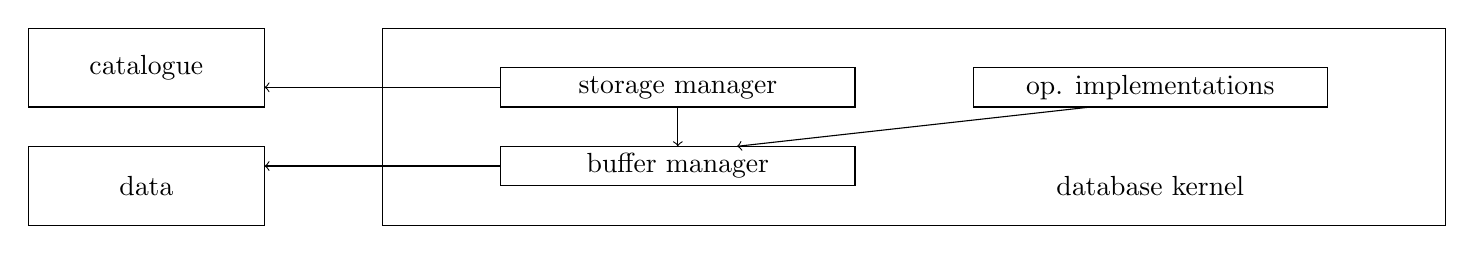
\begin{tikzpicture}[x=1.5cm, y=0.5cm]
                        \draw
                        (0, 0) -- (9, 0) -- (9, -5) -- (0, -5) -- cycle
                        (1, -1) -- (4, -1) -- (4, -2) -- (1, -2) -- cycle
                        (5, -1) -- (8, -1) -- (8, -2) -- (5, -2) -- cycle
                        (1, -3) -- (4, -3) -- (4, -4) -- (1, -4) -- cycle
                        (5, -1) -- (8, -1) -- (8, -2) -- (5, -2) -- cycle
                        (-3, 0) -- (-1, 0) -- (-1, -2) -- (-3, -2) -- cycle
                        (-3, -3) -- (-1, -3) -- (-1, -5) -- (-3, -5) -- cycle;

                        \node at (2.5, -1.5) {storage manager};
                        \node at (2.5, -3.5) {buffer manager};
                        \node at (6.5, -1.5) {op. implementations};
                        \node at (-2, -1) {catalogue};
                        \node at (-2, -4) {data};
                        \node at (6.5, -4) {database kernel};
                        \draw
                        (6, -2) edge[->] (3, -3)
                        (2.5, -2) edge[->] (2.5, -3)
                        (1, -1.5) edge[->] (-1, -1.5)
                        (1, -3.5) edge[->] (-1, -3.5);
                    \end{tikzpicture}
                \end{center}
                The \textbf{buffer manager} manages disk-resident data.
                It maps unstructured files (large 'blobs of bytes') to structured tables for reading and writing.
                Since DBs don't trust OSs, it makes sure files have a fixed size, and it also safely writes data to disk when necessary.
                It also writes in \textbf{open (for writing) pages}.
                An example implementation is as follows;
                \begin{lstlisting}
                    class BufferManager;
                    class Table {
                        BufferManager& bufferManager;
                        string relationName = "Employee";

                        public
                            void insert(Tuple t) {
                                bufferManager.getOpenPageForRelation(relationName).push_back(t);
                                bufferManager.commitOpenPageForRelation(relationName);
                            }

                            vector<Tuple> findTuplesWithAttributeValue(int attribute, AttributeValue value) {
                                vector<Tuple> result;
                                auto pages = bufferManager.getPagesForRelation(relationName);
                                for (size_t i = 0; i < pages.size(); i++) {
                                    auto page = pages[i];
                                    for (size_t i = 0; i < page.size(); i++) {
                                        if (page[i][attribute] == value) {
                                            result.push_back(page[i]);
                                        }
                                    }
                                }
                                return result;
                            }
                    }

                    struct BufferManager {
                        using Tuple = vector<AttributeValue>;
                        using Page = vector<Tuple>;

                        size_t tupleSize;
                        map<string, vector<Tuple>> openPages;
                        map<string, vector<string>> pagesOnDisk; // maps one relation to many pages on disk (filenames)
                        size_t numberOfTuplesPerPage();

                        vector<Tuple>& getOpenPageForRelation(string relationName);
                        void commitOpenPageForRelation(string relationName);
                        vector<Page> getPagesForRelation(string, relationName);
                    }

                    vector<Tuple>& BufferManager::getOpenPageForRelation(string relationName) {
                        return openPages[relationName]; // creates one if needed
                    }

                    void BufferManager::commitOpenPageForRelation(string relationName) {
                        while (openPages[relationName].size() >= numberOfTuplesPerPage(tupleSize)) {
                            vector<Tuple> newPage;

                            // move overflowing tuples to new page
                            while (openPages[relationName].size() > numberOfTuplesPerPage(tupleSize)) {
                                newPage.push_back(openPages[relationName].back());
                                openPages[relationName].pop_back();
                            }

                            pagesOnDisk[relationName].push_back(writeToDisk(openPages[relationName]));
                            openPages[relationName] = newPage; // contains tuples that didn't fit on disk
                        }
                    }

                    vector<vector<Tuple>> BufferManager::getPagesForRelation(string relationName) {
                        vector<vector<Tuple>> result = { openPages[relationName] };
                        for (size_t i = 0; i < pagesOnDisk[relationName].size(); i++) {
                            result.push_back(readFromDisk(pagesOnDisk[relationName][i]));
                        }
                        return result;
                    }
                \end{lstlisting}
                However, we still need to determine ~numberOfTuplesPerPage~;
                \begin{itemize}
                    \itemsep0em
                    \item \textbf{unspanned pages} \hfill pages like mini-databases
                        \subitem
                            The goal of this is simplicity, and good random access performance; we want to find the record with a single page lookup, given a ~tuple\_id~.
                            When we don't have enough space on a page for another tuple, we will write to disk (even when not full) and obtain a new page.
                            However, we can quite easily infer which page a tuple will be on, since we know how many tuples are on each page.
                            This cannot deal with large records (where the size is larger than a page), nor can we have in-page random access if the records are variable size.
                            \begin{lstlisting}
                                const long pageSizeInBytes = 4096;
                                size_t BufferManager::numberOfTuplesPerPage() {
                                    return floor(pageSizeInBytes / tupleSizeInBytes);
                                }

                                // space consumption of a relation of n tuples;
                                ceil(data.size() / mnumberOfTuplesPerPage())
                            \end{lstlisting}
                    \item \textbf{spanned pages} \hfill optimising for space efficiency
                        \subitem
                            On the other hand, the goal here is to minimise space waste and to support large records.
                            Spanned pages can have tuples existing across pages - this is complicated and also hurts random access performance, since we can no longer easily determine where a tuple is.
                            We can calculate the number of pages per relation as follows;
                            \begin{lstlisting}
                                long dataSizeInBytes = tupleSizeInBytes * data.size();
                                long numberOfPagesForTable = ceil(dataSizeInBytes / pageSizeInBytes);
                            \end{lstlisting}
                            However - we cannot determine the number of tuples per page as this is not constant.
                    \item \textbf{slotted pages} \hfill random access for in-place NSM
                        \subitem
                            This is the most complicated method covered, but is also what is used by most systems.
                            This stores tuples in in-place N-ary format, and stores the tuple count in the \textbf{page header} (at the start of the page).
                            Offsets are also stored to every tuple, which are filled in from the \textbf{end} of the page (hence the index of the first tuple is the last item in the page and so on).
                            Offsets need to be typed large enough to address page;
                            \begin{itemize}
                                \itemsep0em
                                \item ~byte~s for pages smaller than 256 bytes
                                \item ~short~s for pages smaller than 65,536 bytes
                                \item ~int~s for pages smaller than 4 gigabytes
                            \end{itemize}
                \end{itemize}
                Some disk-based database systems also keep a dictionary per page, which solves the problem of variable sized records (and allows for duplicate elimination, at the granularity of a single page, as previously mentioned).
                A global dictionary is not used as it will lead to more accesses.
\end{document}